\documentclass{beamer}


\graphicspath{ {pictures/} }

\usetheme{Boadilla}

\title{Distracted Driver Detection}
\subtitle{HLCV Project}
\author[Reyes, Schaefer, Tonsen, Weber]{Guillermo Reyes \\
	 Daniel Schaefer \\
	 Marc Tonsen \\
 Dominik Weber\\}
 \institute[]{Saarland University}
\date{25.07.2016}



\begin{document}
	\begin{frame}
		\titlepage
	\end{frame}


    \begin{frame}{Motivation}
		\frametitle{Motivation}
        \textbf{Distraction-affected crashes 2013:}\\
        \vspace{0.5cm}
        According to U.S. Department of Transportation and the National Highway Traffic Safety Administration \cite{knuthwebsite}
		\begin{itemize}
            \item 10\% of all fatal crashes
			\item 18\% of all injury crashes
		\end{itemize}
        were reported as distraction-affected crashes.\\
        % In 2013 there were over 3000 people killed and over 400.000 injured in motor vehicle crashes involving distracted drivers.\\
        \begin{itemize}
            \item 3.000 people killed
            \item 400.000 injured
        \end{itemize}
        in motor vehicle crashes involving distracted drivers.\\
		\vspace{0.5cm}
		% -> distraction-detection is a really important topic!
		$\Rightarrow$ Simple cameras combined with CV algorithms are non-intrusive and relatively cheap! 
        % compared to for example specialized sensors
	\end{frame}
	
	
	\begin{frame}
		\frametitle{Task}
		Kaggle CV Competition: State Farm Distracted Driver Detection \\
		Given a picture of the driver we have to predict the class it belongs to
		
		\begin{columns}
			\begin{column}{0.5\textwidth}
				\begin{itemize}
					\item c0: safe driving
					\item c1: texting - right
					\item c2: talking on the phone - right
					\item c3: texting - left
					\item c4: talking on the phone - left
					\item c5: operating the radio
					\item c6: drinking
					\item c7: reaching behind
					\item c8: hair and makeup
					\item c9: talking to passenger			
				\end{itemize}
			\end{column}
			\begin{column}{0.5\textwidth}  %%<--- here
				\begin{center}
					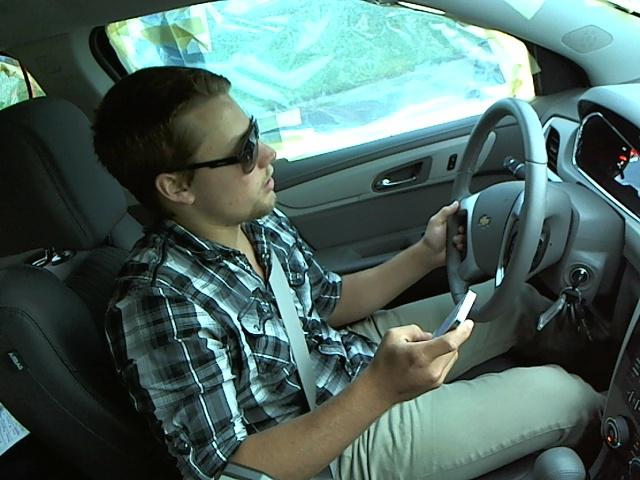
\includegraphics[width=0.9\textwidth]{img_6}
				\end{center}
			\end{column}
		\end{columns}
	\end{frame}

    \begin{frame}
		\frametitle{Classes}
			\begin{center}
                \quad drinking \quad \quad \quad \quad \quad \quad  texting left\\
				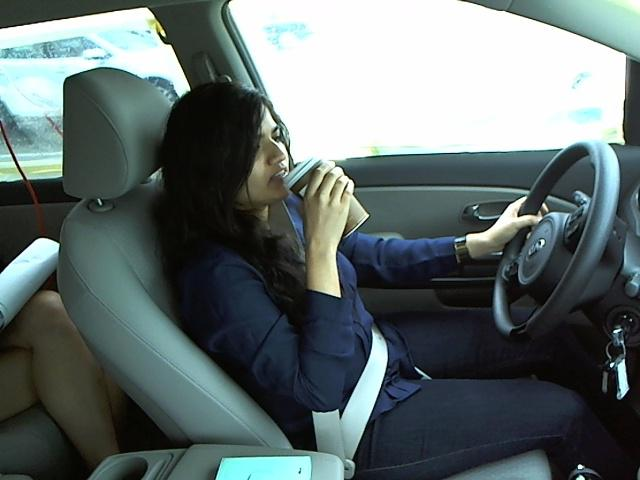
\includegraphics[width=4cm]{img_0} \vspace{0.1cm}
				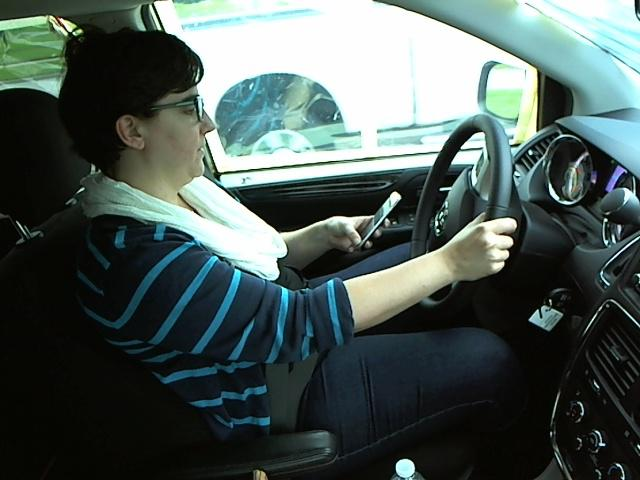
\includegraphics[width=4cm]{img_5} \\
				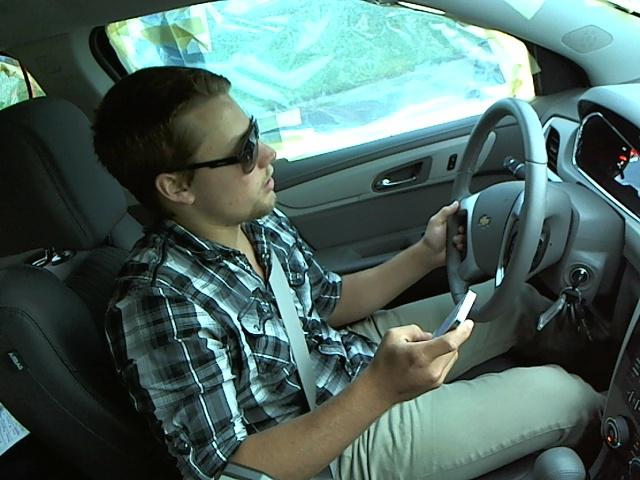
\includegraphics[width=4cm]{img_6}\vspace{0.1cm}
				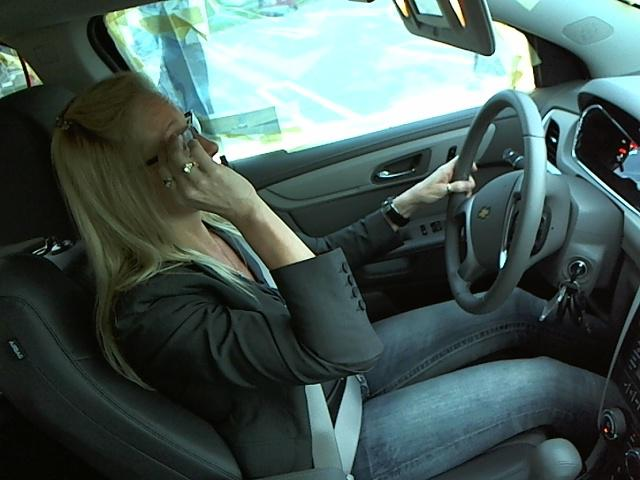
\includegraphics[width=4cm]{img_26}\\
                \quad texting right \quad \quad \quad \quad hair and makeup
			\end{center}
	\end{frame}
	
	\begin{frame}
		\frametitle{Classes}
		\begin{center}
            talking to passenger \quad \quad \quad operating radio \quad \\
			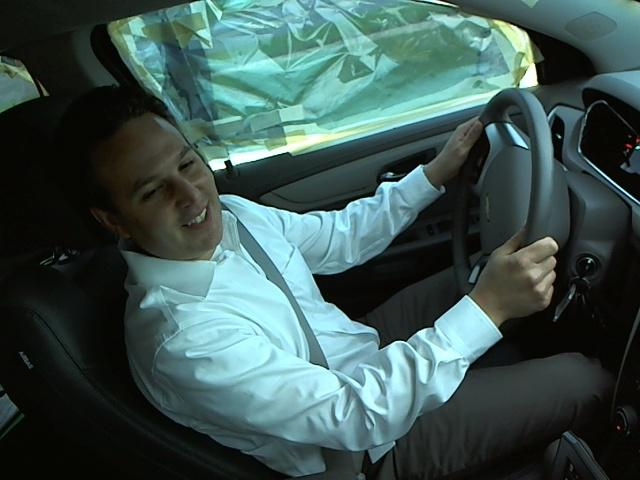
\includegraphics[width=4cm]{img_19} \vspace{0.1cm}
			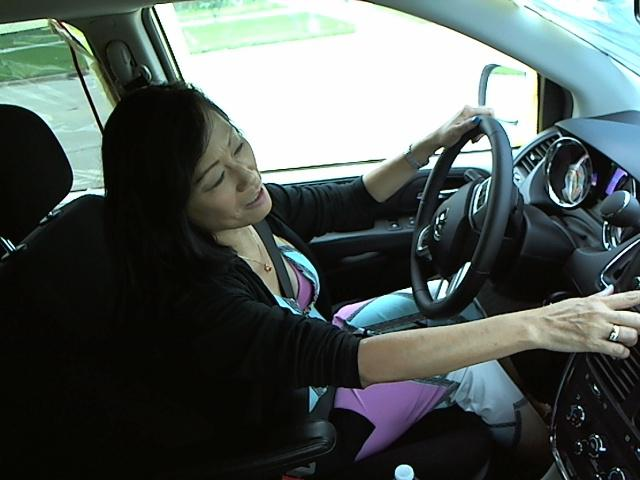
\includegraphics[width=4cm]{img_56} \\
			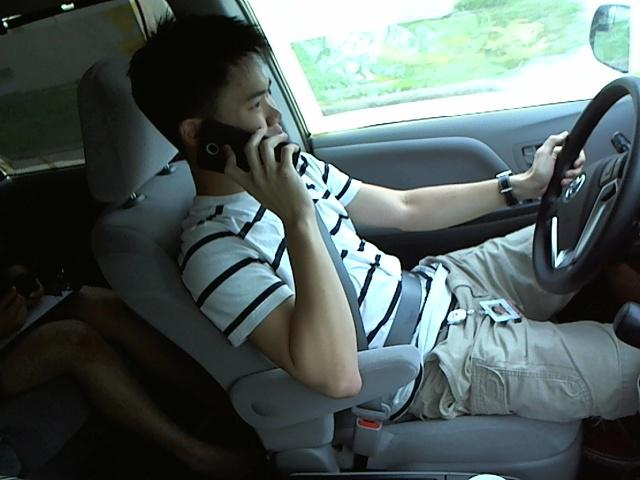
\includegraphics[width=4cm]{img_94}\vspace{0.1cm}
			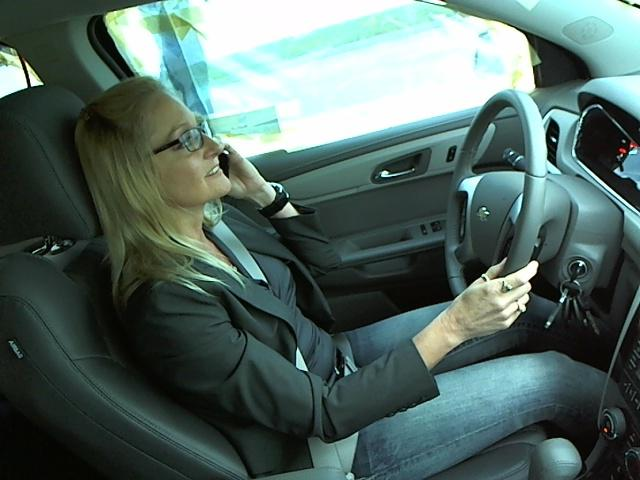
\includegraphics[width=4cm]{img_14}\\
            talking on the phone right \quad  talking on the phone left \quad \\
		\end{center}
	\end{frame}
	
	\begin{frame}
        \frametitle{Classes}
		\begin{center}
            save driving \quad \quad \quad \quad \quad \quad \quad reaching behind\\
			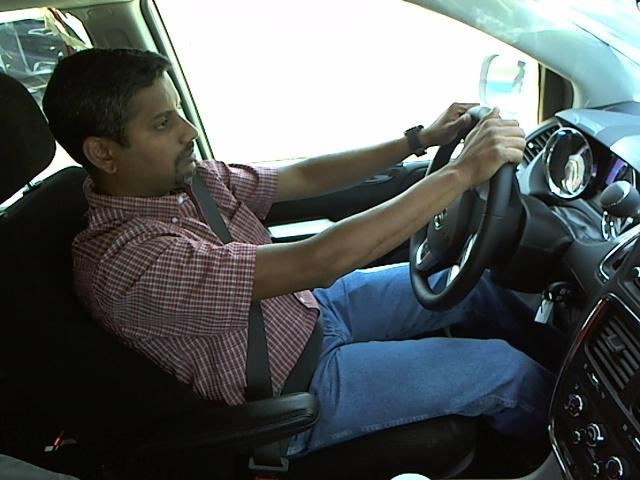
\includegraphics[width=5cm]{img_34} \vspace{0.1cm}
			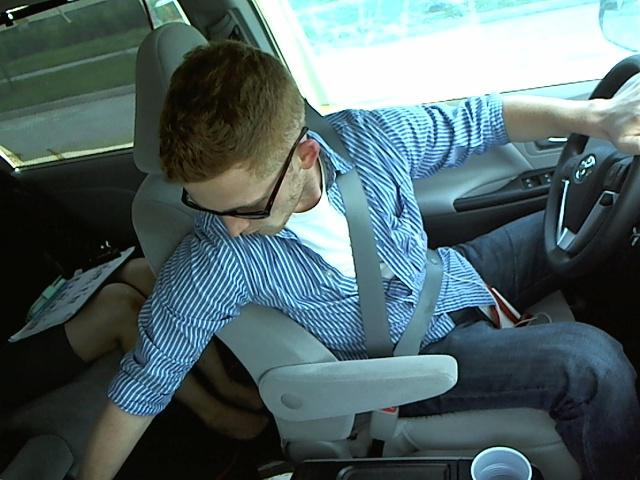
\includegraphics[width=5cm]{img_81} 
		\end{center}
	\end{frame}



    \begin{frame}{Dataset}
        \frametitle{Dataset}
        \begin{columns}
        \begin{column}{0.5\textwidth}
            \begin{itemize}
                \item 
                    around 2000 pictures per class
                    % in the available training set, which we also used for testing
                    % because we don't have the classes of the test set and we didn't
                    % want to rely on the online evaluation of the testset containing
                    % almost 80.000 pictures -> more control
                \item 
                    26 different participants
                    % with each participant having roughly the same amount of pictures
                    % per class.
                \item 
                    4 different cars (with different camera angles)
                \item 
                    different light situations
                \item 
                    sometimes very minor differences between certain classes
             \end{itemize}
        \end{column}
        \begin{column}{0.5\textwidth}
            \begin{center}
                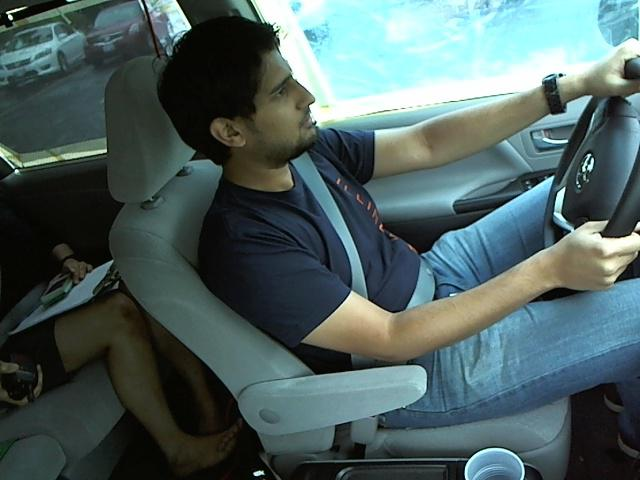
\includegraphics[width=0.8\textwidth]{c0}\\
                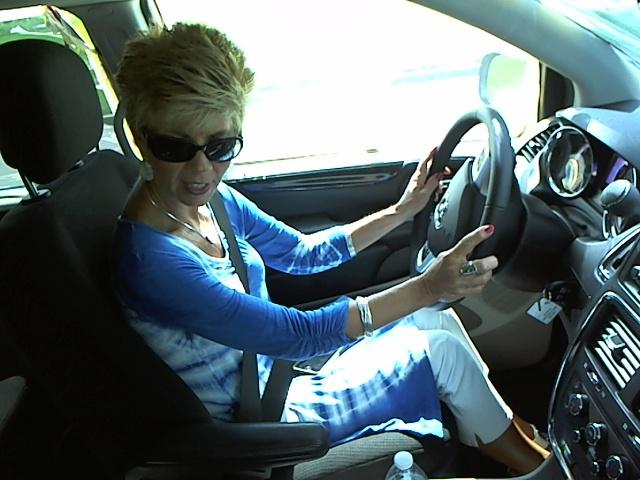
\includegraphics[width=0.8\textwidth]{c_0_angle2_passenger}
                % both of these pictures are being contained in the c0 (save driving)
                % class.
            \end{center}
        \end{column}
        \end{columns}
    \end{frame}


	\begin{frame}
		\frametitle{Related Work}
		
		\begin{columns}
			\begin{column}{0.75\textwidth}
                \textbf{Driver-Distraction Detection:}
				\begin{itemize}
					\item Datasets mostly from cameras with frontal-views, captures in artificial environments  \cite{itsc:bergasa2008}
					\item Some approaches with specialized sensors (RGBD cameras etc.) \cite{Ragab2014}
					\item Mostly rely on gaze-tracking or head-pose estimation \cite{Dorazio} \cite{6957817}
				\end{itemize}		
                \textbf{Activity Recognition}
					\begin{itemize}
						\item Often use different sensors (wearable sensors, smartphones) \cite{6258525} \cite{6365160}
						\item Camera based ones rely on continues video \cite{1315249} \cite{1430826}
					\end{itemize}	
                \vspace{0.5cm}
                $\Rightarrow$ current methods are not applicable in our case!
			\end{column}
			\begin{column}{0.25\textwidth}  %%<--- here
				\begin{center}
					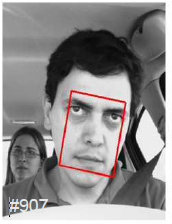
\includegraphics[width=0.9\textwidth]{frontal-view-dataset} \\
					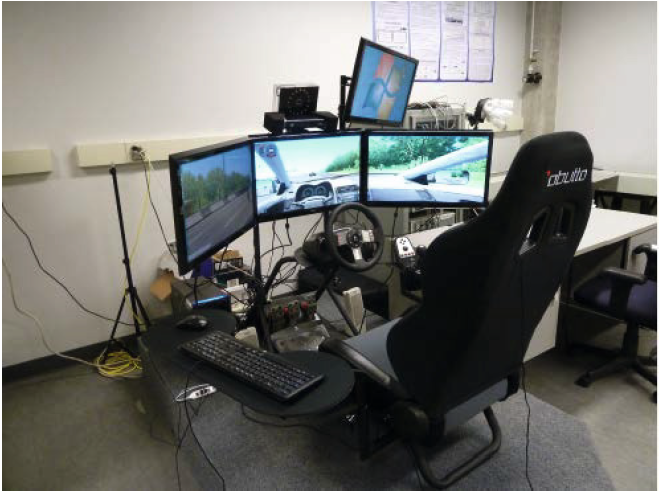
\includegraphics[width=0.9\textwidth]{RanForSim}
				\end{center}
			\end{column}
		\end{columns}
	\end{frame}

    
	\begin{frame}[allowframebreaks]
		\frametitle{References} 
		\nocite{*} 
		\bibliographystyle{amsalpha} 
		\bibliography{references} 
	\end{frame}
	
	\medskip

	
	
\end{document}
